\clearpage\begingroup\SourceLeaf{35b}\HistoricalHead{30}{L}{PHYSIK. BRIEFWECHSEL.}
\begin{center}
[8.]\\[.7em]
\textsc{Gauss} an \textsc{Schumacher}. Göttingen, 4. Februar 1837.
\par\medskip\rule{.78\textwidth}{.35pt}\par
{\small [Briefwechsel zwischen \textsc{Gauss} und \textsc{Schumacher} III, Altona 1860, S. 142, 143.]}\par
\rule{.78\textwidth}{.35pt}
\end{center}
\noindent .\ .\ .\ .\ .\ .\ .\ .\ .\ .\ .\ .\ .\ .\ .\ .\ .\ .\ .\ .\ .
\par\noindent\hspace*{\parindent}In Beziehung auf die Waagen von der gewöhnlichen Einrichtung mit drei
Schneiden, möchte ich mir wohl noch Ihre und eventuell Herrn \textsc{Repsolds}
Belehrung über einen Umstand ausbitten, den ich geneigt bin für sehr wichtig,
und wie eine Hauptursache [anzusehen], warum bei sonst vortrefflichen Waagen
die \textls[120]{wiederholten} Wägungen oft viel grössere Unterschiede geben, als man
\clearpage\SourceLeaf{36}\HistoricalHead{31}{R}{GAUSS AN SCHUMACHER.}
\noindent nach den regelmässigen Schwingungen und der Schärfe, womit sich jedesmal
deren Mittel bestimmen lässt, erwarten sollte.

Diese ist der \textls[120]{Parallelismus der Schneiden}. Fehlt daran etwas, so
wird daraus, dass nach dem Auslösen das Tragstück\textsuperscript{*})\begingroup\renewcommand{\thefootnote}{}\footnotetext{\begin{minipage}{.94\linewidth}\noindent\begin{minipage}[t]{.80\linewidth}\vspace{0pt}\textsuperscript{*}) So nenne ich die Stahlplatte, die auf der Schneide schwebt. Hat
dieses Stück einen bei den Künstlern recipirten Namen, so verbinden Sie
mich \textls[120]{sehr} durch Anzeige desselben.\end{minipage}\hfill
\begin{minipage}[t]{.17\linewidth}\vspace{0pt}\centering
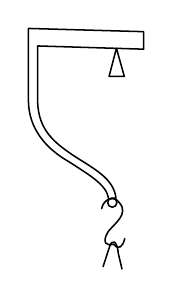
\begin{tikzpicture}[x=.0023in,y=-.0023in,line width=.55pt,line cap=round,line join=round]
\draw (30,30)--(280,37)--(280,75)--(50,68)--(50,190)
 .. controls (52,252) and (88,279) .. (128,306)
 .. controls (171,334) and (215,355) .. (220,398)
 --(204,400)
 .. controls (201,369) and (157,345) .. (119,320)
 .. controls (68,291) and (31,248) .. (30,188)--cycle;
\draw (221,73)--(205,134)--(238,134)--cycle;
\draw (212,408) circle [radius=10];
\draw (189,421) .. controls (192,402) and (215,389) .. (228,409)
 .. controls (248,433) and (217,453) .. (203,471)
 .. controls (188,496) and (200,503) .. (215,498)
 .. controls (226,513) and (235,503) .. (239,486);
\draw (192,547)--(205,507)
 .. controls (212,482) and (223,493) .. (225,518)--(233,552);
\end{tikzpicture}\end{minipage}\end{minipage}}\endgroup\ sich nie wieder \textls[120]{genau
so} wie vorher, auflegt, ein abgeändertes Moment, also ein anderes Resultat
erfolgen.

Die \textls[120]{gewöhnlichen} Mittel, womit die Mechanici solchen Parallelismus
prüfen, sind aber meiner Meinung nach sehr roh. \textsc{Weber} und \textsc{Meierstein}
sagen mir, dass sie bloss längs den Schneiden nach Einem entfernten Object
visiren, und daraus auf etwaige Divergenz schliessen. Ich würde dem Augenmaass
keinen Vorwurf machen, wenn man bei einem so rohen Verfahren über
einen Grad fehlte.

Es ist mir so, als hätten Sie mir schon voriges Jahr einmahl über diesen
Umstand geschrieben und gesagt, dass \textsc{Repsold} diesen Parallelismus durch
Messung der Distanzen der Schneiden prüfte. Ich habe alle Ihre aufbewahrten
Briefe vom vorigen Jahre wieder durchgemustert, kann aber die betreffende
Stelle nicht wieder finden. Vielleicht ist der Brief bei mir verlegt oder verloren.
Jedenfalls verstehe ich die Art, wie die Messungen, und mit welchen
Mitteln sie gemacht sind, so noch nicht. Ich bitte recht dringend, mir
darüber vollständigen Aufschluss zu geben.

Ich bin nemlich vor 8 Tagen auf eine eigenthümliche Methode gekommen,
solchen Parallelismus zu prüfen. Um sie \textls[120]{genau} auszuführen, muss ich erst
einiges dazu machen lassen. Ein roher Versuch gab mir aber an \textsc{Repsolds}
Waage eine Divergenz von \(\tfrac{1}{4}\) Grad zwischen der mittlern und linken Schneide.
Unter Anwendung der gehörigen Vorkehrungen glaube ich diese Grösse auf
einen kleinen Bruchtheil Einer Minute bestimmen zu können.

Ich würde gern geneigt sein mein Verfahren, sobald ich etwas reifere
\clearpage\SourceLeaf{37}\HistoricalHead{32}{L}{PHYSIK. BRIEFWECHSEL.}
\noindent Versuche damit gemacht habe, in unsern g[elehrten] A[nzeigen] bekannt zu
machen. In der Societät habe ich vor 8 Tagen, bei Gelegenheit einer Vorlesung
von \textsc{Weber} über Waagen von verschiedenen neuen Einrichtungen, einen
Vortrag gehalten[\textsuperscript{*})]\begingroup\renewcommand{\thefootnote}{}\footnotetext{[\textsuperscript{*}) Siehe Göttingische Gelehrte Anzeigen vom 13. März 1837, Werke V, S. 511; der Vortrag von \textsc{Gauss} im Anschluß an die Vorlesung \textsc{Webers} fand am 28. Januar 1837 statt.]}\endgroup. Allein ich möchte gern vorher die Mittel, deren \textsc{Repsold}
sich bedient, vollständig kennen.\quad .\ .\ .\ .\ .\ .\ .\ .\ .\ .\ .\ .\ .\ .\ .\ .\ .\ .\ .\ .\ .\ .
\clearpage\endgroup
